\section{Introduction}
\label{sec:introduction}

\subsection{Research Background and Motivation}
Knowledge graph (KG) quality control involves two linked decisions: which defects to repair and which rules to acquire. A repair may require a validator that is not yet available. Acquiring more rules consumes resources, and a rule that covers few remaining defects may have little immediate value. This dependence motivates a scheduler that responds to the current graph and available rules.

Rules also require a source of new candidates. Expert constraints capture known requirements, while text can suggest additional type, hierarchy, and procedural constraints. Large language models (LLMs) offer a way to propose such candidates. Turning a proposal into a useful validator requires executable semantics, a compatible vocabulary, and evidence of detection quality.

We study reinforcement learning (RL) for allocating a finite budget between graph and rule operations, together with two ways to elicit rule candidates from text. The central link is an executable validator: acquiring it changes which repairs are available, and repairing the graph changes the value of later acquisitions.

Our evaluation follows this link in three stages. First, a fixed validator registry lets us compare learned scheduling, simple policies, and reward choices under the same graph transitions. Second, a paired generation archive measures what deletion completion and augmentation expansion contribute. Third, direct execution and document-based development tests check whether generated candidates supply useful repair actions. The trained policy results come from the first stage; the third stage uses fixed schedules to assess the conditions for learning with generated-rule arrivals.

\subsection{Contributions of This Paper}
We make three contributions:
\begin{enumerate}
    \item \textbf{An executable graph--rule co-optimization environment.} We define fourteen observed features, eight graph and rule actions, feasibility masks, and a cost-aware reward. Graph actions change stored records, and rule actions change the validators available for later repairs.
    \item \textbf{A trained Double-DQN policy and matched control study.} An action-level audit shows how a count penalty can discourage useful relation repairs by charging for temporary duplicates. Forty retrained neural policies, ten fitted one-step baselines and reserved test scenarios compare three fixed penalties using reference-fact and structural metrics. Matched ablations under the rate reward test graph features, rule features, action masking and acquisition cost. The studies identify reward sensitivity, the contribution of masking, and the remaining performance gap to simple controls.
    \item \textbf{Dual-strategy rule generation with traceable evaluation.} Deletion completion and augmentation expansion propose candidates in a shared schema. We compare candidate diversity at equal call budgets, distinguish declarations from constraints, and trace exact typed-rule execution back to the archived response. Fixed-schedule execution and source-evidence development tests then locate the gap between candidate diversity and useful repair coverage.
\end{enumerate}

Figure~\ref{fig:rl_framework} summarizes the framework. The policy receives fourteen features describing graph quality, rule quality, remaining defects, remaining budget, and active rule fractions. A feasibility mask controls action selection. The selected operation changes the environment, which recomputes quality and reward. Separate diagnostic probes inspect one-step transitions; evaluated policies use only the current observation and mask.

\begin{figure*}[t]
    \centering
    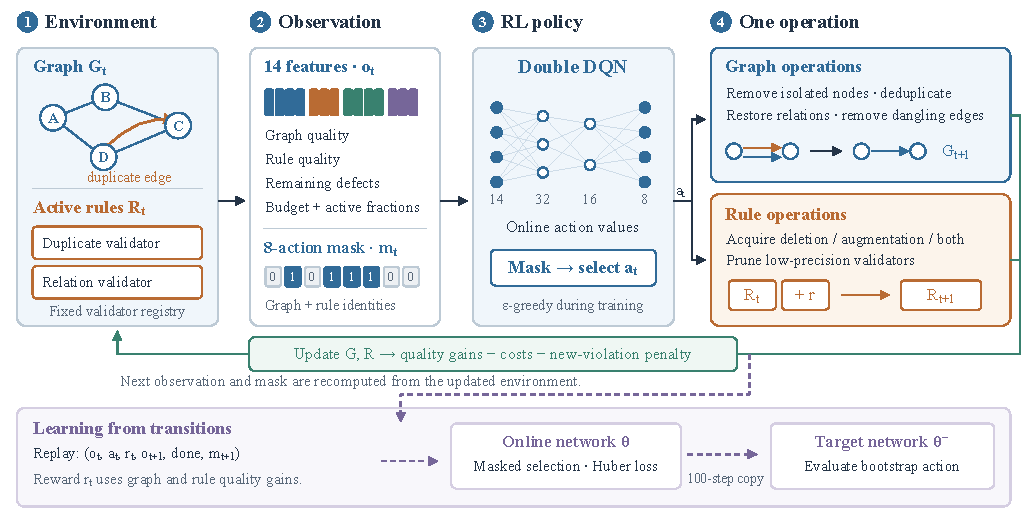
\includegraphics[width=0.96\textwidth]{figure/method/cooptimization.pdf}
    \caption{RL graph--rule co-optimization. The environment supplies fourteen observed features and an eight-action feasibility mask. The policy selects one graph or rule operation; the environment then updates quality and reward. The lower band shows replay-based Double-DQN training. Miniature graphs and mask entries illustrate the mechanism. The scheduling loop uses a fixed validator registry; text-derived candidate generation is shown in Figure~\ref{fig:dual_strategy}.}
    \label{fig:rl_framework}
\end{figure*}

\subsection{Paper Organization}
Section~\ref{sec:related_work} reviews related work. Section~\ref{sec:methodology} presents the scheduling model and rule-generation procedures. Section~\ref{sec:experiments} follows the three evaluation stages, then discusses their joint implications. The appendices provide protocols, detailed execution records, and supporting repair-layer checks.
